\chapter{Probabilistic Connectivity of Tree Networks}
\begin{quote}

In this chapter, we consider the connectivity problems introduced in Chapter 1 on probabilistic graphs that have the topology of a tree. We present a dynamic programming algorithm to solve the $SR$-$CONN$ problem on such networks. The algorithm is designed to solve the more restricted $AR$-$CONN$ problem while incurring only a small overhead compared to a specialized algorithm for solving the problem. Since the $SR$-$CONN$ problem is the most general problem among the four problems defined in Chapter 1, it follows that the algorithm presented in this chapter can solve the remaining three probabilistic connectivity problems. Results in this chapter appear in our work in \cite{Tree2014}.
\end{quote}

\section{System Model}
\label{sec:ch3sm}
We recall that a probabilistic graph $G=(V,E_G,Loc,p)$ is specified by the following:
\begin{itemize}[noitemsep]
\item $V=V_{sense}\cup V_{relay}$ the set of nodes in a given UWSN $G$
\item $E_G(x[i],y[j])=1$ if and only if the two nodes $x$ and $y$ can reach each other when located anywhere in their respective rectangles $x[i]$ and $y[j]$. This restriction results in computing lower bounds on the solution since we ignore cases where $x$ and $y$ can reach each other if they are located in some (but not all) positions in their respective rectangles.
\item $Loc(v)$ is the locality set of node $v$. 
\item $p_v(i)$ is the probability that node $v$ is located at grid rectangle $v[i]$. 
\end{itemize}
We say that the probabilistic graph $G$ has the topology of a conventional tree $T=(V,E_T)$ if whenever $E_G(x[i],y[j])= 1$
then $(x,y) \in E_T$.
%
Note that the definition allows two nodes $x$ and $y$ to be adjacent in
$T$, and yet they can take positions, say $x[i]$ and $y[j]$, such that
$E_G (x[i],y[j])= 0$.
%
Thus, each state $S$ of $G$ gives a subgraph of $T$.\\
\nwline
In any such tree network $T$, one may safely delete a relay node
$x \in V_{relay}$ that appears as a leaf node without changing the problem
solution. 
%
This observation holds since relay nodes are relevant only if they
connect some sensor node to the sink $s$.
%
We henceforth assume, without loss of generality, that the input network $G$ has no relay leaf.\\


We also recall that in the $AR$-$CONN$ problem, a state is {\em operating} if the sink $s$
can reach all sensor nodes in $V_{sense}$.
%
In the $SR$-$CONN$ problem, a state $S$ is {\em operating} if
the sink node $s$ can reach a subset having at least $n_{req}$ sensor nodes.
%
Let $\textbf{S}$ be the set of all operating states $S$ of a given
$AR$-$CONN$ or $SR$-$CONN$ problem then the required solution is given by $\sum_{S \in \textbf{S}} Pr(S)$.
\section{Overview of the Algorithm}
The algorithm (Function $Conn$ in Figure ~\ref{alg:Conn}) employs a
dynamic programming approach.
%
It takes as input an instance $(G,n_{req})$ of the $SR$-$CONN$ problem,
and a tree $T=(V,E_T)$ on the set $V$ of nodes with no relay leaves.
%
The function computes the exact solution $Conn(G,n_{req})$ of the given
instance.

The pseudo-code uses syntax similar to $C/C\mbox{++}$ languages. In particular, we use $x \starEqual y$ (or, $x \plusEqual y$) to mean $x=x*y$ (respectively, $x=x+y$).
We consider $T$ as a tree rooted at the sink $s$. Each node $y$ in $T$ except $s$ has a parent node $x$ on the unique path from $y$ to the root $s$.
%
Each such node $y$ is a root of a subtree, denoted $T_y=(V_y,E_{T_y})$, obtained by
removing the link $(y, parent(y))$ from $T$.

%----------------------------
%There will be a figure here
%---------------------------------
\begin{example}
\normalfont
Figure \ref{fig:es31} illustrates a tree network where $|V_{sense}|=7$ and $|V_{relay}|=3$ nodes. $Children(x_2)=\{y_1,y_2,y_3\}$ and subtree $T_{y_3}$ has nodes $\{y_3,z_3,z_4\} \blacksquare$.
\end{example}
\begin{figure}[!htb]
\centering
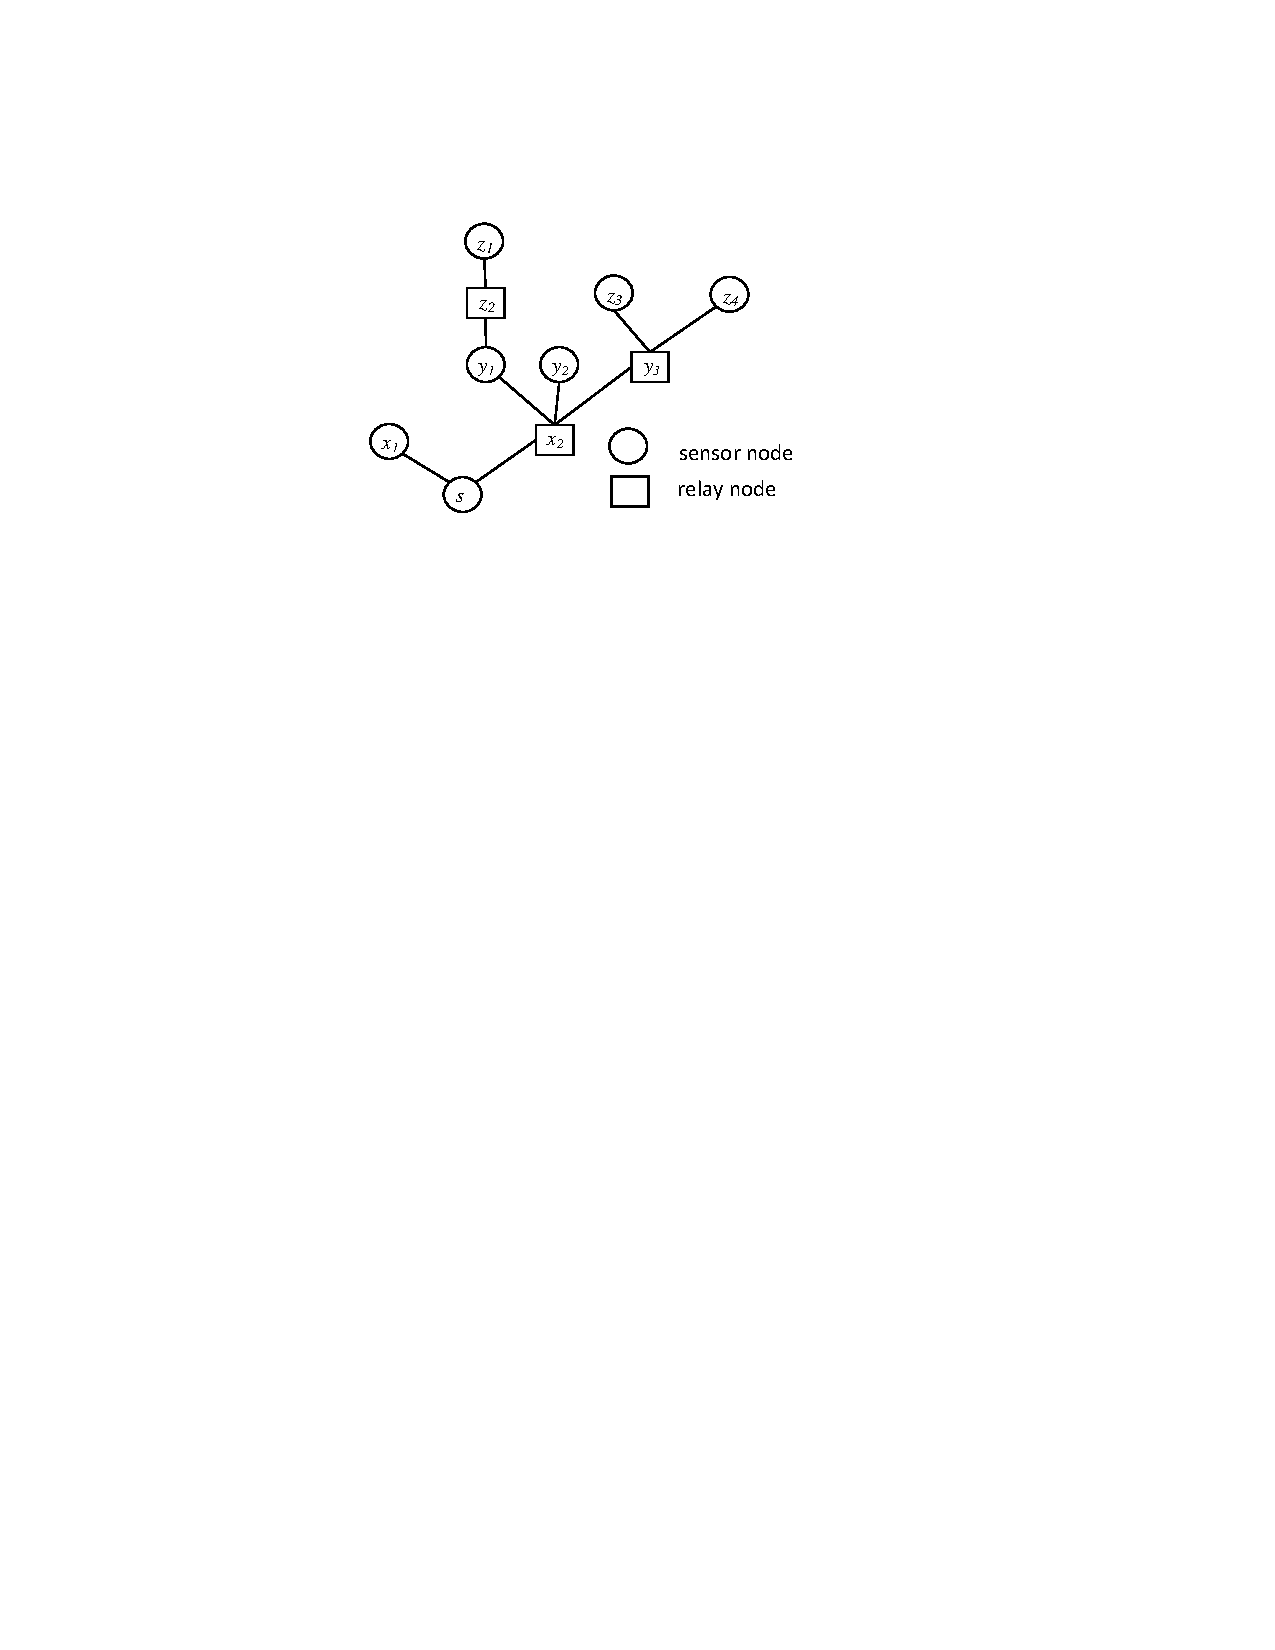
\includegraphics[width=3 in, height=1.8 in]{Ch4f1.pdf}
 \caption{ A tree network}
\label{fig:es31}
\end{figure}

The key variables and data structures in the function are as follows.

\begin{itemize}[noitemsep]
\item	$type(x)$:
	For any node $x$, $type(x)= 0$ if $x$ is a relay node,
	and $type(x)= 1$ if $x$ is a sensor node.

\item	$n_{sense}(X)$: The number of sensor nodes in a given subset  of nodes $X\subseteq V$. We use $n_{sense}$ for $n_{sense}(V)$.


\item   $n_{relay}(X)$: The number of relay nodes in a given subset of nodes $X\subseteq V$. We use $n_{relay}$ for $n_{relay}(V)$.

\item $n(X)=n_{sense}(X) + n_{relay}(X)$.

\item $n_{sense,min}(X)$: The minimum number of sensor nodes in a given subset $X\subseteq V$ that should be connected to the sink in any operating state of the overall network. So,\\
\centerline{
$n_{sense,min}(X)=max(0,n_{req}-n_{sense}(\overline{X}))$
}

\nwline
where $\overline{X}=V\setminus X$ (the complement set of $X$). So $n_{sense}(\overline{X})$ is the number of available sensor nodes not in $X$. Consequently, $n_{req}-n_{sense}(\overline{X})$, if non-negative, is the minimum number of sensor nodes of $X$ required in any operating state of the network. 

\begin{example}
\normalfont
In figure \ref{fig:es31}, consider node $x_2$. Using the above notation, $n(V_{x_2})=8$ where $n_{sense}(V_{x_2})=5$ and $n_{relay}(V_{x_2})=3$. Assuming $n_{req}=5$ in an instance of the $\SRCONN$ problem then $n_{sense,min}(V_{x_2})=3=n_{req}-n_{sense}(\{s,x_1\})=5-2$ $\blacksquare$
\end{example}
The dynamic program associates with each node $x$ a table, denoted $R_x$. Initially, $R_x$ contains information derived from node $x$ only. Subsequently, the algorithm performs $n-1$ iterations. Each iteration of the main loop in Step 2 identifies
	a non-sink leaf node $y$ in the current tree whose parent is denoted $x$. 
	The function then processes, and then deletes node $y$. Processing of node $y$ is done by updating summary information in table $R_x$ using information in table $R_y$. Subtree $T_y$ is considered one part of the tree $T_x$ that has been processed thus far. We also need the following definitions and notation.

\item	$DCH(x)$:	In any iteration, each node $x$ may have some of its children
	processed and deleted.
	We denote such set of $x$'s \textbf{deleted children} by $DCH(x)$.

\item	Tables $R_x$ (and $R'_x$):
	Each node $x \in V$ is associated with a table $R_x$.
	The table stores {\em key-value} mappings.
	%
	Each key is a pair $(i,count)$ where $i$ is a possible location
	index of $x$, and $count$ is a number of sensor nodes that are
	descendants of $x$ (including $x$ itself) in the graph processed
	thus far.
	%
	Roughly speaking, at any iteration of the main loop,
	$R_x(i,count)$ is the probability of obtaining a state over
	the subset of nodes in $T_x$ processed in previous iterations
	where $x[i]$ reaches exactly $count$ sensor nodes in such subset of
	$T_x$. 

\end{itemize}
\begin{example}
\normalfont
In figure \ref{fig:es31}, consider node $x_2$ and its associated tree $T_{x_2}$. Assume that the algorithm has processed and deleted nodes in subtree $T_{y_1} \mbox{ and } T_{y_2}$. Thus, $DCH(X)=\{y_1,y_2\}$, and all nodes in $V_{y_1}\cup V_{y_2}=\{z_1,z_2,y_1,y_2\}$ have been deleted. Now assume that $n_{req}=5$. After deleting nodes in  $V_{y_1}\cup V_{y_2}$, the algorithm computes\\
\centerline{
$n_{sense,min}(\{x_2\}\cup V_{y_1}\cup V_{y_2}) \begin{array}[t]{l}
=n_{req}-n_{sense}(\{s,x_1,y_3,z_3,z_4\})\\
=5-4\\
=1
\end{array}
$
}
This value is the minimum number of sensor nodes in the set $X=\{x_2\}\cup V_{y_1}\cup V_{y_2}$ required to be connected to the sink in any operating state of the overall graph. $\blacksquare$
\end{example}
% ------------------------------
    % --------------- Function E2P ---------------
    \begin{figure}[htbp]
    % \begin{figure}[!ht]
    \small
\begin{center}
\fbox{
    \begin{minipage}[t]{6 in}
    \renewcommand{\baselinestretch}{1}
    %
    {\bf Function $\fConn (G, T, \nReq)$}
\nwline
	{\bf Input:}
	\begin{minipage}[t]{5in}
	An instance of the $SR$-$CONN$ problem where $G$ has a tree
	topology $T$ with no relay leaves
	\end{minipage}
%
\nwline
	{\bf Output:}
	\begin{minipage}[t]{5in}
	$Conn(G, \nReq)$
	\end{minipage}
	\\
%
%\nwline
%	{\bf Notation:}
%	\begin{minipage}[t]{2.75in}
%	\end{minipage}
% --------------------
   \nwline
% initialization
   1.  \begin{minipage}[t]{5in}
       {\bf foreach} (node $x$ and a valid location index $i$) \\
       \{ \\
         \iin{0.20} set $R_x(i, type(x) )= 1$ \\
         %\iin{0.20} $n_{x,min}= \min (0, \nReq - (n_{sense} - n_{x,sense}) )$ \\
       \}
       \end{minipage}
       \\
   \nwline       
% main loop
   2.  \begin{minipage}[t]{5in}
       {\bf while} ($T$ has at least 2 nodes) \\
       \{
       \end{minipage}
       \\
   3.  \iin{0.20} \begin{minipage}[t]{5 in}
   		  Let $y$ be a non-sink leaf of $T$, and $x= parent(y)$
		  \end{minipage}
		  \\
   4.  \iin{0.20} \begin{minipage}[t]{5 in}
   		  {\bf foreach} (key $(i,count) \in R_y$)
		       $R_y (i,count) \starEqual p_y(i)$
		  \end{minipage}
		  \\
   5.  \iin{0.20} \begin{minipage}[t]{5in}
   		  set $R'_x= \phi$
		  \end{minipage}
		  \\
   6.  \iin{0.20} \begin{minipage}[t]{5in}
   		  {\bf foreach} (pair of keys
		       		$\begin{array}[t]{l}
				 (i_x, count_x) \in R_x \mbox { and }
		   		 (i_y, count_y) \in R_y)
				 \end{array}
				$ \\ 
		  \{
		  \end{minipage}
		  \\
   7.  \iin{0.40} \begin{minipage}[t]{5 in}
   		  $count= \min (\nReq, count_x + count_y)$
		  \end{minipage}
		  \\
%   8.  \iin{0.40} \begin{minipage}[t]{5 in}
%   		  $count_{x,min}= \begin{array}[t]{l}
%		  		  type(x) + n_{y,min} + 
%		       	   	  \sum_{z \in \DCH(x)} n_{z,min}
%				  \end{array}$
%		  \end{minipage}
%		  \\
  8.  \iin{0.40} \begin{minipage}[t]{5 in}
   		  {\bf if} ($count < n_{sense,min}(\{x\}\cup V_y \cup_{z\in DCH(x)} V_z)$) {\bf continue} 
		  \end{minipage}
		  \\
   9.  \iin{0.35} \begin{minipage}[t]{5in}
   		  $R'_x (i_x,count) \plusEqual$ 
		  	$\begin{array}[t]{l}
			 R_y(i_y,count_y) \times 
			 R_x(i_x,count_x) \times 
			 E_G(x[i_x], y[i_y])
		  	 \end{array}$
		  \end{minipage}
		  \\
       \iin{0.40} \} \\
   10. \iin{0.20} \begin{minipage}[t]{5 in}
       		  set $R_x= R'_x$; remove $y$ from $T$
		   \end{minipage}
		   \\
       \iin{0.15} \} \\
   11. \begin{minipage}[t]{6 in}
       return $\sum_{s[i] \in \loc(s)} R_s(i,\nReq) * p_s(i)$
       \end{minipage}
       \\
    \end{minipage}	
}
\end{center}
    \normalsize
    %
    \caption{Pseudo-code for function $\fConn$}
    \label{alg:Conn}
\vspace*{-0.1in}
    \end{figure}
    % ------------------------------
\section{Main Steps}
Step 1 initializes table $R_x$ for each node $x$ as follows.
%
For each possible location index $i$ of $x$, set $R_x(i, count=1)= 1$
if $x$ is a sensor node.
Else ($x$ is a relay node), set $R_x(i, count=0)= 1$.
%
%Step 1 also initializes $n_{x,min}$.


Steps 2-10 form the main loop of the function.
The loop iteratively finds a leaf node $y$ that is not the sink $s$, 
processes node $y$, and then removes $y$ from the tree $T$.
%
Processing a node $y$ with parent $x$ is done as follows.

Step 4 updates each entry $R_y (i,count)$ by multiplying the entry
with $p_y(i)$.
%
As can be seen, this update operation is done in the iteration that ends by
removing $y$.
%
Step 5 initializes the temporary table $R'_x$ to empty.


Steps 6-9: the loop in Step 6 performs a {\em cross product} of tables
$R_x$ and $R_y$, storing the result in table $R'_x$.
%
In the cross product, each pair of possible keys $(i_x, count_x)$
and $(i_y, count_y)$ are processed.
%
More specifically, suppose that $x[i_x]$ can reach $count_x$ sensor nodes
in the part of $T_x$ processed thus far with probability $R_x(i_x,count_x)$.
%
Also, suppose that $y[i_y]$ can reach $count_y$ sensor nodes
in $T_y$ with probability $R_y(i_y,count_y)$.
%
Thus, if $x[i_x]$ reaches $y[i_y]$ (i.e., $E_G(x[i_x],y[i_y])$= 1)
then $x[i_x]$ can reach a total of $count= count_x + count_y$ nodes.


If $count > \nReq$ then Step 7 truncates $count$ to $\nReq$.
%
On the other hand, if $count < n_{sense,min}(\{x\}\cup V_y  \cup_{z\in DCH(x)} V_z)$ (i.e., $count$ is below the
minimum number of nodes required to construct an operating state) then
Step 8 skips Step 9 and starts a new iteration.
%
Step 9 updates the probabilities accumulated in $R'_x(i_x,count)$. 


After exiting the main loop, the current tree $T$ contains only the
sink node $s$. Step 11 computes the solution $Conn(G,\nReq)$ from
the table $R_s$ associated with the sink $s$.
% ------------------------------

\section{Correctness}

To prove correctness, we first introduce the following notation and
definitions.
%
For a given node $x$, and iteration $r \in [1,n-1]$ of the main loop
in Step 2, we have the following:
%
\begin{itemize}
\item	$\DCH (x,r)$:
	The set of $x$'s deleted children at the start of iteration $r$.

\item	$V_{x,deleted,r}$ ($= \bigcup_{y \in \DCH(x,r)} V_y$):
	The set of $x$'s deleted descendants at the start of iteration $r$.
\end{itemize}
%
For brevity, we omit $r$ when the iteration number is not important, or
understood by the context.


In the following definitions, $x$ is any node in $T$,
$i$ is a possible location index of $x$, and  $V_{x,delete}$ is
the set of deleted descendants associated with $x$ at the start of some
iteration.

\begin{enumerate}[noitemsep]
\item[{\bf [D1]}]
    Let $S$ be a state over nodes in $\{ x \} \bigcup V_{x,delete}$.
    The {\em type} of $S$ is a pair $(i,count)$ where
    %
    \begin{itemize}
    \item   $x$ is at location $x[i]$
    \item   If $count = \nReq$ then the number of sensor nodes connected to
    	    $x[i]$ in $S$ is $\geq \nReq$
    \item   Else ($count < \nReq$), then the number of sensor nodes
    	    connected to $x[i]$ is $< \nReq$
    \end{itemize} 	   
\end{enumerate}

\begin{enumerate}
\item[{\bf [D2]}]
    We say that table $R_x$ is {\em complete} with respect to a given
    set $V_{x,delete}$ if the following conditions hold:
    %
    \begin{enumerate}
    \item  For each key $(i,count)$ in $R_x$, $R_x(i,count)$ is
    	   the probability of obtaining states over
	   $\{ x[i] \} \bigcup V_{x,delete}$ of type $(i,count)$.
	   (Before multiplying by $p_x(i)$, the probability is conditioned
	   on $x$ being at location $x[i]$).
    \item  Each key $(i,count)$ not in $R_x$ does not contribute to
    	   computing the solution $Conn(G,\nReq)$.
    \end{enumerate}
\end{enumerate}

\nwline
We now show the following theorem.

\begin{theorem} \label{thm:correctness}
\normalfont
    At the start of each iteration of the main loop in Step 2,
    if $x$ is a node in the current tree $T$ then table $R_x$ is complete
    with respect to the associated set $V_{x,delete}$ of deleted nodes.
\end{theorem}

\nwline
{\bf Proof.}
\nwline
{\bf Loop initialization:}
At the start of the 1st iteration, $T$ contains all nodes $V$, and
each node $x$ has $V_{x,delete}= \emptyset$.
%
Node $x$ in location $x[i_x]$ is associated with one state of type
$(i_x,count_x= 0)$ if $x$ is a relay node, or type
$(i_x,count_x= 1)$ if $x$ is a sensor node.
%
For each such state type, Step 1 correctly sets $R_x(i,count)$.

\nwline
{\bf Loop maintenance:}
Assume the theorem holds for all possible iterations $r$, where $r \leq n-2$.
We show that it holds in iteration $r+1$.
%
Let $y$ be the leaf node deleted in iteration $r$, and $x= parent(y)$.
$R_x$ is the only relevant table that may have changed between iterations
$r$ and $r+1$ (table $R_y$ is also changed but node $y$ is deleted at the end of the iteration).
%
Thus, it suffices to show that $R_x$ is complete with respect to
$\{ x \} \bigcup V_{x,delete,r+1}$ at the start of iteration $r+1$.
%
To this end, we note the following in iteration $r$:
%
\begin{itemize}[noitemsep]
\item  Step 4: this step adjusts the probability of each state type
       $(i,count)$ in $R_y$ by taking into account $p_y(i)$.
\item  Step 6: this loop exhaustively generates all state types over the
       set $V_y \bigcup V_{x,delete,r}$ where $V_y$ is all nodes of
       the subtree rooted at node $y$.
\item  Step 8: this step discards all state types that can not be extended
       (by adding sensor nodes from the unprocessed part of the tree)
       to satisfy the $\nReq$ requirement.
\item  Step 9: this step updates the probability of $R'_x(i_x,count)$ by
       adding the right hand side when states of type $(i_x, count)$
       can be extended to operating states.
\end{itemize}
$\blacksquare$

Following an argument similar to the loop maintenance argument, one can
show that at Step 11, table $R_s$ associated with the sink node is
complete with respect to all nodes $V$ in the network.
%
Thus, the function returns the required solution $Conn(G, \nReq)$.

% ------------------------------

\section{Running Time}

Let $n$ be the number of nodes in $G$, and $\ell_{max}$ be the maximum
number of locations in the locality set of any node.

% ----------
\begin{theorem}
\normalfont
    Function $\fConn$ solves the $\SRCONN$ problem in
    $O(n \cdot n_{req}^2  \cdot \ell_{max}^2)$ time
\end{theorem}

\nwline
{\bf Proof.}
We note the following.
\begin{itemize}[noitemsep]
\item   Step 1: storing the tree $T$ requires $O(n)$ time.

\item	Step 2: the main loop performs $n-1$ iterations.
	Each of Steps 3, 5, and 10 can be done in constant time.

\item	Step 4: this loop requires $O(\nReq \cdot \ell_{max})$ time.

\item	Step 6: this loop requires $O(n_{req}^2 \cdot \ell_{max}^2)$ iterations.
	Steps 7, 8, and 9 can be done in constant time.
\end{itemize}
Thus, the overall running time is determined by the main loop that
requires $O(n \cdot n_{req}^2  \cdot \ell_{max}^2)$ time.
$\blacksquare$
% ----------
%
\nwline
\begin{theorem}
\normalfont
    Function $\fConn$ solves the $\ARCONN$ problem in
    $O(n \cdot \ell_{max}^2)$ time.

    % Overall: $O(n \cdot \ell_{max} + n \cdot \ell_{max}^2)$
\end{theorem}

\nwline
{\bf Proof.}
It suffices to show that the main loop requires the above time.
%
In the $\ARCONN$ problem, $\nReq= |V_{sense}|$, and all sensor nodes
in any subtree $T_y$ should be connected to the root $y$ in any
operating state.
%
So, in any iteration of the main loop, each table $R_y$ contains keys
$(i,count)$ for only one value of $count$ (the maximum value obtainable
from descendants of $y$ processed and removed thus far).
%
That is, the maximum length of any table is $\ell_{max}$ independent
of $\nReq$.
%
This gives the running time shown in the theorem. 
$\blacksquare$
\section{Simulation Results}
We present performance results of the algorithm with results on partial 2-trees and 3-trees in the next chapter. The tree algorithm is empirically fast. The running time is typically
less than 50 millisecond for the tested tree networks of size $\leq 20$ nodes.
In contrast, the algorithm for 2-trees and 3-trees may require time in the order of minutes to solve
a network with 15 nodes.
\section{Concluding Remarks}
Quantifying the likelihood that a sufficient number of sensor nodes is connected to a sink node in a given UWSN is
a challenging problem for networks with semi-mobile and mobile nodes. Here, we adopt a flexible probabilistic
graph model to formulate a class of parametrized network connectivity problems. The problem setting allows the network
to utilize both sensor nodes and relay nodes. For scenarios where the model is exact, our devised algorithm shows that the exact probabilistic connectivity can be computed efficiently for tree-like networks.
